%-----------------------------------------------------------------------------%
\chapter{\topikSatu}
%-----------------------------------------------------------------------------%

%-----------------------------------------------------------------------------%
\section{Eksperimen}
%-----------------------------------------------------------------------------%
Pada bagian ini kami melakukan 2 eksperimen untuk mengamati perilaku \textit{block} dan \textit{thread} pada \textit{kernel} dan mengamati pengaruh ukuran data terhadap eksekusi \textit{kernel}.

\subsection{Eksperimen Perilaku Thread dan Block 1} 

Bagian ini adalah eksperimen untuk mengamati perilaku \textit{block} dan \textit{thread} pada \textit{kernel}.

\subsubsection{Deskripsi Program}

Program yang digunakan merupakan hasil modifikasi program dari \textit{slide} \"Intro to Cuda\".  Program dimodifikasi agar dapat menerima argumen untuk menentukan jumlah \textit{block} dan jumlah \textit{thread} per \textit{block}.

	\begin{lstlisting}
	blockgrid [ukuran array] [thread/block] [block]
	\end{lstlisting}

Program akan menjalankan 3 buah \textit{kernel}.  \textit{Kernel} pertama akan mengisi array dengan angka konstan 9, \textit{kernel} kedua akan mengisi array dengan \textit{block id}, dan \textit{kernel} ketiga akan mengisi array dengan \textit{kernel id}.

	\begin{lstlisting}
	__global__ void kernel1( int *a )
	{
	    int idx = blockIdx.x * blockDim.x + threadIdx.x;
	    a[idx] = 9;
	}
	
	__global__ void kernel2( int *a )
	{
	    int idx = blockIdx.x * blockDim.x + threadIdx.x;
	    a[idx] = blockIdx.x;
	}
	
	__global__ void kernel3( int *a )
	{
	    int idx = blockIdx.x * blockDim.x + threadIdx.x;
	    a[idx] = threadIdx.x;
	}
	\end{lstlisting}
	
\subsubsection{Hasil Eksperimen}

Berikut adalah hasil eksperimen dengan variasi jumlah \textit{block}.

\begin{figure}
	\centering
	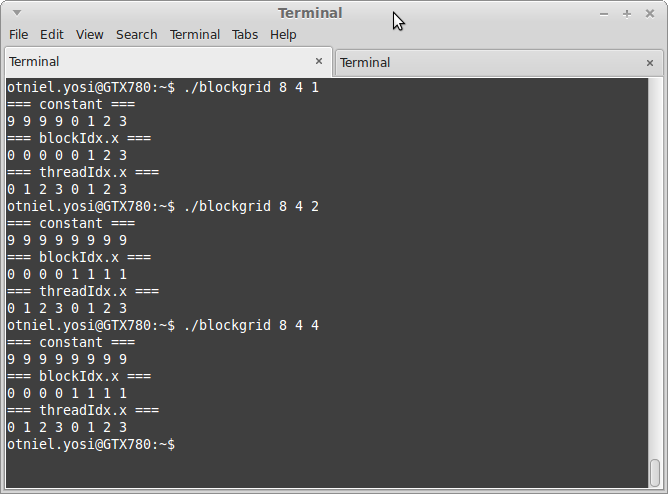
\includegraphics[width=1\textwidth]
	{pics/block1}
	\caption{Hasil eksperimen dengan variasi block 1}
	\label{fig:block_demo1}
\end{figure}  

\begin{figure}
	\centering
	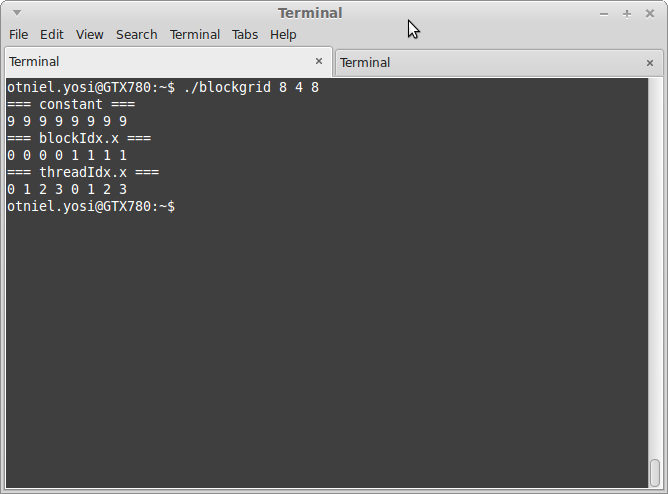
\includegraphics[width=1\textwidth]
	{pics/block2}
	\caption{Hasil eksperimen dengan variasi block 2}
	\label{fig:block_demo2}
\end{figure}

Berikut adalah hasil eksperimen dengan variasi jumlah \textit{thread} per \textit{block}.

\begin{figure}
	\centering
	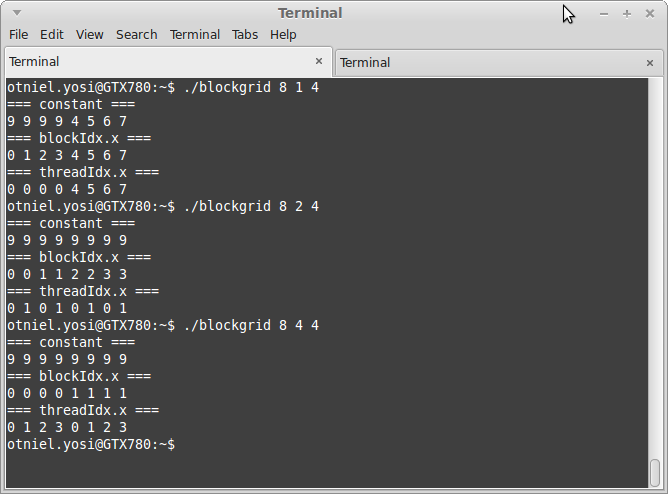
\includegraphics[width=1\textwidth]
	{pics/grid1}
	\caption{Hasil eksperimen dengan variasi thread per block 1}
	\label{fig:block_demo1}
\end{figure}  

\begin{figure}
	\centering
	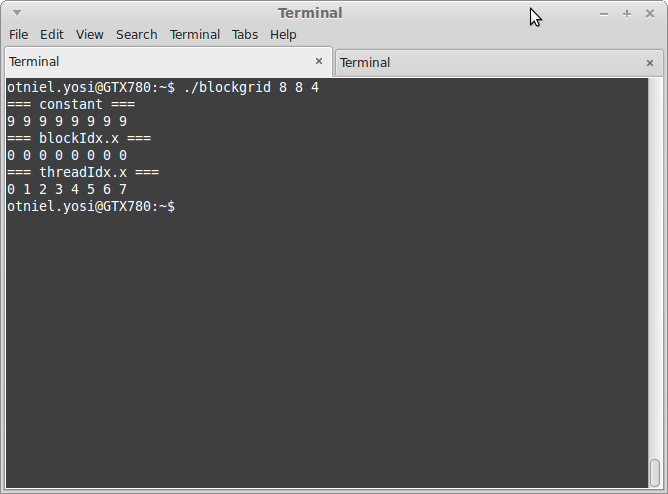
\includegraphics[width=1\textwidth]
	{pics/grid2}
	\caption{Hasil eksperimen dengan variasi thread per block 2}
	\label{fig:block_demo2}
\end{figure}

Dari hasil eksperimen terlihat bahwa konfigurasi yang benar untuk menjalankan program adalah jumlah \textit{thread} per \textit{block} dikalikan jumlah \textit{block} yang digunakan tidak melebihi jumlah data yang diproses.  Saat program diberi parameter dengan jumlah data 8, jumlah \textit{thread} per \textit{block} 4, dan jumlah \textit{block} 2 terlihat program dijalankan oleh 2 \textit{block} dengan id 0 dan 1 dan pada tiap \textit{block} terdapat \textit{thread} dengan id 0 sampai 3.  Namun saat jumlah \textit{block} ditingkatkan dengan jumlah data dan \textit{thread} per \textit{block} yang sama, progam tetap menampilkan 2 \textit{block} dengan id 0 dan 1 karena 2 \textit{block} tersebut sudah cukup untuk menangani jumlah data yang digunakan.

\subsection{Eksperimen Perilaku Thread dan Block 2} 

Bagian ini adalah eksperimen untuk mengamati pengaruh ukuran data terhadap eksekusi \textit{kernel}.

\subsubsection{Deskripsi Program}

Program yang digunakan sesuai dengan lampiran pada soal tugas.  Program dimodifikasi agar dapat menerima masukan berupa ukuran array dan banyaknya iterasi yang akan dilakukan.

\subsubsection{Hasil Eksperimen}

Eksperimen pertama dilakukan dengan memasukkan ukuran array maksimal dan banyaknya iterasi.  Ukuran array yang digunakan di setiap iterasi akan diacak saat iterasi berlangsung.  Banyaknya \textit{block} yang digunakan adalah 4 dan banyaknya \textit{thread} per \textit{block} adalah ukuran array dibagi banyaknya \textit{block}.  Berikut adalah hasil eksperimennya.

\begin{figure}
	\centering
	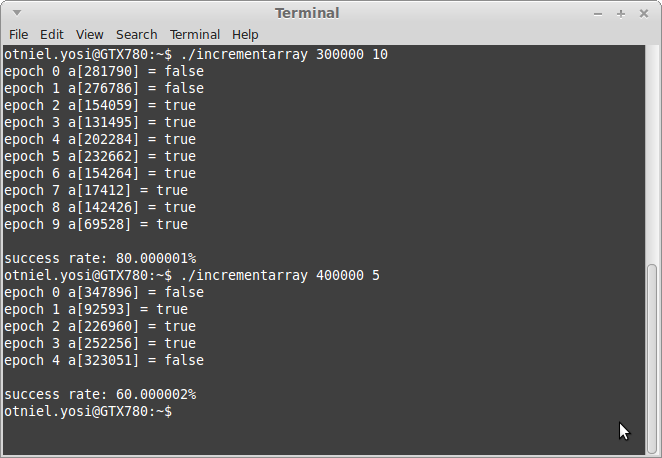
\includegraphics[width=1\textwidth]
	{pics/incrementarray}
	\caption{Hasil eksperimen 1}
	\label{fig:inc_demo1}
\end{figure}

Terlihat program mengeluarkan nilai \textit{false} pada ukuran array diatas 270000.  Program akan mengeluarkan nilai \textit{false} ketika ukuran array lebih dari atau sama dengan 262140 karena 262140/4 adalah 65535 yang merupakan batas maksimum banyaknya \textit{block} dalam grid 1D.

Eksperimen kedua dilakukan hampir sama dengan eksperimen pertama tetapi banyaknya \textit{thread} per \textit{block} disesuaikan dengan iterasi (iterasi ke-i maka banyaknya \textit{thread} per \textit{block} adalah i ).  Berikut adalah hasil eksperimennya.

\begin{figure}
	\centering
	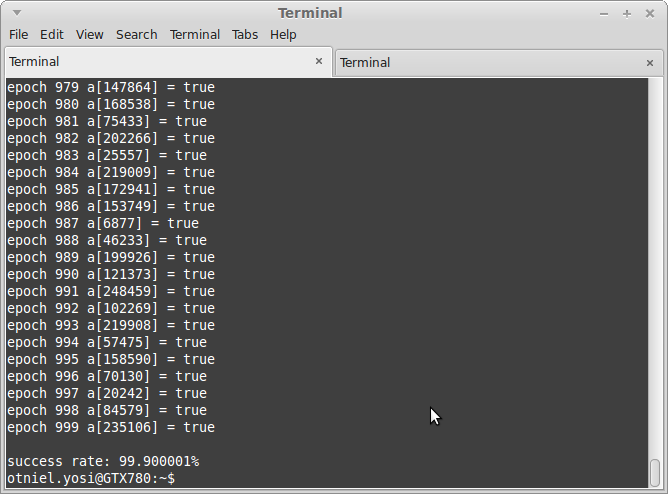
\includegraphics[width=1\textwidth]
	{pics/incarray_blockvar_1000}
	\caption{Hasil eksperimen 2a}
	\label{fig:inc_demo1}
\end{figure}

\begin{figure}
	\centering
	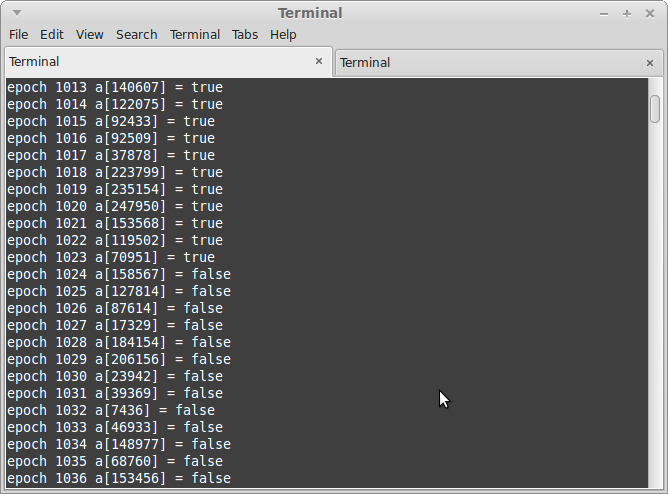
\includegraphics[width=1\textwidth]
	{pics/incarray_blockvar_1500}
	\caption{Hasil eksperimen 2b}
	\label{fig:inc_demo1}
\end{figure}

Terlihat program mengeluarkan nilai \textit{false} pada saat jumlah \textit{block} lebih dari atau sama dengan 1024.  Nilai tersebut adalah nilai maksimum banyaknya \textit{thread} yang bisa digunakan dalam suatu \textit{block}.

%-----------------------------------------------------------------------------%
\section{Kesimpulan}
%-----------------------------------------------------------------------------%

\begin{itemize}
	\item Setiap \textit{thread} dalam \textit{block} dan setiap \textit{block} dalam \textit{grid} memiliki id yang unik.
	\item Dengan menggunakan kombinasi \textit{thread id} dan \textit{block id} kita bisa mendapatkan index yang unik di setiap \textit{kernel}.
	\item \textit{Device} memiliki batasan dalam hal jumlah memory, banyaknya \textit{block}, dan banyaknya \textit{thread} per \textit{block} yang bisa digunakan.
	\item Konfigurasi yang melebihi batasan akan mengakibatkan kesalahan akses memori yang mengakibatkan kegagalan program.  
\end{itemize}
